% !TeX root = RJwrapper.tex
\title{sugarglider: Create glyphmaps of spatio-temporal data}


\author{by Maliny Po and Dianne Cook}

\maketitle

\abstract{%
(An abstract of less than 150 words.)
}

\hypertarget{introduction}{%
\section{Introduction}\label{introduction}}

\begin{verbatim}
Note: use similar terminology as cubble & glyph-maps. Add a quick start (quick guide on how to use the sugarglider package)
\end{verbatim}

\hypertarget{literature-review}{%
\section{Literature Review}\label{literature-review}}

\hypertarget{glyph-maps}{%
\subsubsection{Glyph Maps}\label{glyph-maps}}

\begin{verbatim}
(Desperately need more resources)
\end{verbatim}

\begin{itemize}
\item
  Glyph maps are a specific type of multivariate glyph plots where each spatial location is represented by a glyph that encapsulates data measured over time at that location. As detailed in \href{https://vita.had.co.nz/papers/glyph-maps.pdf}{Hadley Wickham's} paper, glyph maps are particularly effective for uncovering both local and global structures, emphasizing temporal relationships within the data. These maps utilize small glyphs or icons to represent multiple data values at each location, extending the concept of glyphs which are traditionally used to display multivariate data.
\item
  Challenges with Faceted Maps and Spatio-Temporal Animations: While faceted maps and spatio-temporal animations are useful for highlighting spatial patterns, they often fall short in adequately showcasing temporal trends. To overcome this, a transformation technique is employed which utilizes principles of linear algebra to convert temporal coordinates (minor coordinates) into spatial coordinates (major coordinates). This transformation is implemented in packages such as \href{https://cran.r-project.org/web/packages/GGally/GGally.pdf}{GGally} and \href{https://www.jstatsoft.org/article/view/v110i07}{cubble}, facilitating a more integrated approach to spatio-temporal data visualization.
\item
  The R package \href{https://www.jstatsoft.org/article/view/v110i07}{cubble} introduces an innovative cubble class designed to efficiently organize spatial and temporal variables. This dual structure allows for separate or combined manipulation of these variables while maintaining synchronization. A spatial cubble object is constructed from distinct spatial and temporal tables through the function make\_cubble(), requiring the specification of three attributes: key, index, and coords. This functionality not only simplifies the data wrangling process but also enhances the analytical capabilities when dealing with complex datasets.
\end{itemize}

\hypertarget{extending-ggplot2-with-ggproto}{%
\subsubsection{Extending ggplot2 with ggproto}\label{extending-ggplot2-with-ggproto}}

\begin{verbatim}
 Diversify your resources a bit :((
\end{verbatim}

\begin{itemize}
\tightlist
\item
  Elegant Graphics for Data Analysis: The architecture of ggplot2 is fundamentally based on the ggproto system of object-oriented programming. Initially, ggplot2 utilized the proto system, developed by Grothendieck, Kates, and Petzoldt in 2016, for object-oriented tasks. This system, described in detail in the \href{https://cran.r-project.org/web/packages/proto/proto.pdf}{Proto package documentation},
  outlines that proto is an S3 subclass of the R environment class, implying single inheritance and mutable state characteristic of all environments. Proto objects are created and modified using the proto function which sets the parent environment, evaluates expressions, and handles lazy evaluation of arguments.
\end{itemize}

However, as the need for an official extension mechanism in ggplot2 grew, the limitations of the proto system became apparent, leading to the adoption of ggproto. This transition is well-documented in Hadley Wickham's book, \href{https://ggplot2-book.org/}{ggplot2: Elegant Graphics for Data Analysis}, which also introduces how to utilize ggproto objects to extend ggplot2 functionalities.

The creation of a new ggproto object is facilitated by the ggproto() function, which requires the name of the new class and an existing ggproto object from which it will inherit. For instance, to introduce a new statistical transformation, one might create a ggproto that inherits from \texttt{Stat} and \texttt{Geom.} However, merely creating a ggproto object does not make it accessible or useful to the end user.

(Example from ggplot2-book.org)

\begin{verbatim}
NewObject <- ggproto(
  `_class` = NULL, 
  `_inherits` = NULL
)
\end{verbatim}

To bridge this gap, the creation of a layer function is necessary. An example is the \texttt{new\_stat()} function, which follows a consistent format: setting defaults in the function arguments, and calling layer(), which handles the distribution of these arguments into either geom parameters, stat parameters, or aesthetics. This function exemplifies the methodology to create functional and user-accessible components in ggplot2.

(Example from ggplot2-book.org)

\begin{verbatim}
new_stat <- function(mapping = NULL, data = NULL, 
                       geom = "geometry", position = "identity", 
                       na.rm = FALSE, show.legend = NA, 
                       inherit.aes = TRUE, ...) {
  layer(
    stat = NewStat, 
    data = data, 
    mapping = mapping, 
    geom = geom, 
    position = position, 
    show.legend = show.legend, 
    inherit.aes = inherit.aes, 
    params = list(na.rm = na.rm, ...)
  )
}
\end{verbatim}

While developing ggplot2 extensions, it may seem intuitive to encapsulate extensions as new geoms, as they are frequently used by users to add layers to a plot. However, the diversity in ggplot2's capabilities often stems more from the variety in statistical transformations (stats) than merely geometric objects (geoms), suggesting a nuanced approach in designing extensions that effectively enhance the plotting system.

\hypertarget{software}{%
\section{Software}\label{software}}

\begin{verbatim}
Check out:  https://journal.r-project.org/articles/RJ-2023-013
Note: collect all the technical part in one section
\end{verbatim}

\texttt{sugarglider} provides ggplot2 extensions to create glyph maps that visualize seasonal aspects of spatio-temporal data with geom\_glyph\_ribbon() and geom\_glyph\_segment().

Designed to visualize seasonal aspects of spatio-temporal data, sugarglider has the capability to display glyphs with ribbon or segment geometry based on the combination of x\_major and y\_major. Figure \ref{fig:comparison-plot} highlights the package's versatility. The code for these examples is provided below and can be summarised as consisting of the following components. First the glyph plot is created by adding either ribbon or segment geom from ggplot2. For each x\_minor value, geom\_glyph\_ribbon() displays a y interval defined by ymin\_minor and ymax\_minor. Meanwhile, geom\_glyph\_segment() draw a straight line between y\_minor and yend\_minor with respect to x\_minor. An optional global\_rescale argument allow users to control whether rescalling is applied globally across all glyphs or individually for each glyph.

\texttt{add\_ref\_line}, \texttt{add\_ref\_box}, and \texttt{add\_geom\_legend}

\includegraphics{sugarglider_files/figure-latex/comparison-plot-1.pdf}

Furthermore, sugarglider allows various features to be customised:
- \textbf{Scaling of minor values} with-in a grid cell along the x and y dimension.
- \textbf{Rescale} of the value in ploted in each glyph. Determines whether rescaling is applied globally across all glyphs or individually for each glyph.
- \textbf{Width} and \textbf{height} of the glyphs.

The following section will discuss these features and provide examples of their use.

\hypertarget{data-structure}{%
\subsubsection{Data structure}\label{data-structure}}

The first step to creating a glyph plot with sugarglider is to ensure that the data are in supported format. There are 2 data structure to consider Zhang et al. (2024), one of which is compatible with sugarglider. sugarglider exspect data in a long format with temporal and spatial elements.

One dataset provided in the package is the \texttt{aus\_temp} dataset which derives from The National Oceanic and Atmospheric Administration (NOAA) provides comprehensive weather data from numerous stations across Australia. The aus\_temp dataset includes key climate variables, such as precipitation and temperature, recorded at 29 different weather stations throughout 2020. It has spatial elements (longitude, latitude), temporal elements (month) and range of temperature that define the width of ribbon and segment plot.

\begin{verbatim}
glimpse(aus_temp)
\end{verbatim}

\begin{verbatim}
#> Rows: 348
#> Columns: 7
#> $ id    <chr> "ASN00001020", "ASN00001020", "ASN00001020", "ASN00001020", "ASN~
#> $ long  <dbl> 126.3867, 126.3867, 126.3867, 126.3867, 126.3867, 126.3867, 126.~
#> $ lat   <dbl> -14.0900, -14.0900, -14.0900, -14.0900, -14.0900, -14.0900, -14.~
#> $ month <dbl> 1, 2, 3, 4, 5, 6, 7, 8, 9, 10, 11, 12, 1, 2, 3, 4, 5, 6, 7, 8, 9~
#> $ tmin  <dbl> 253.4516, 248.6786, 253.6129, 244.0357, 220.4138, 202.3667, 153.~
#> $ tmax  <dbl> 319.0000, 322.6071, 333.1935, 340.9310, 331.9333, 310.9000, 291.~
#> $ prcp  <dbl> 163.87096774, 162.74074074, 42.00000000, 21.57142857, 0.00000000~
\end{verbatim}

In many cases, analysts may initially receive station data containing geographic location information, recorded variables and their recording periods. They can then query the temporal variables using the stations of interest to obtain the relevant temporal data. Alternatively, analyses may begin as purely spatial or temporal, and analysts may obtain additional temporal or spatial data to expand the result to spatio-temporal. In this case, users can compose cubble objects using functions from cubble packages such as make\_cubble() and pass the new data to sugarglider.

\hypertarget{rescale}{%
\subsubsection{Rescale}\label{rescale}}

sugarglider rescale minor axies (data that are used to plot the individual glyphs) before plotting the glyphs. The purpose of rescaling the value to prepare the data for the linear transformation to map temporal data into a spatial one, which will be explored in the next section. The rescale is controlled by 2 parameters: \texttt{x\_scale} and \texttt{y\_scale}. \texttt{x\_scale} scales each set of minor values within a grid cell along the x-dimension. \texttt{y\_scale} scales each set of minor values within a grid cell along the y-dimension. The default rescale is `identify' which adjust minor axes to to fit within an interval of {[}-1,1{]} using the following equation.

\begin{figure}
\centering
\includegraphics{sugarglider_files/figure-latex/defaultRescale-1.pdf}
\caption{\label{fig:defaultRescale}Default rescale. Additional codes are needed for plotting the base map}
\end{figure}

Users can also change the rescale function by replacing the default value for \texttt{x\_scale} and \texttt{y\_scale} with their own function. In the example code below, we have a custom rescale function that transform value into an interval of {[}0,1{]}.

\begin{figure}
\centering
\includegraphics{sugarglider_files/figure-latex/customRescale-1.pdf}
\caption{\label{fig:customRescale}Custom rescale. Additional codes are needed for plotting the base map}
\end{figure}

With the new rescale functions, we can observe that the ribbon are alot thinner than the previous example. To understand how rescale impact the mapping of temporal data into glyphs, we need to look at the how rescale is applied for both \texttt{geom\_glyph\_ribbon} and \texttt{geom\_glyph\_segemnt} and the spatial temporal transformation for each of these plot type in the following section.

sugarglider also allow user to choose whether rescaling is applied globally across all glyphs or individually for each glyph. This is controlled by an option called \texttt{global\_rescale}. The default for this parameter is \texttt{TRUE}. User can specify for a local rescale by setting \texttt{global\_rescale} to be \texttt{FALSE}. The differences between local and global rescale can be observed in the following example:

\includegraphics{sugarglider_files/figure-latex/unnamed-chunk-5-1.pdf}

sugarglider apply rescaling in multiple steps. First the (\ldots)
For \texttt{geom\_glyph\_ribbon} the rescale is done separately for ymin\_minor and ymax\_minor.

(\ldots\ldots.)

\hypertarget{spatial-temporal-transformation}{%
\subsubsection{Spatial-temporal transformation}\label{spatial-temporal-transformation}}

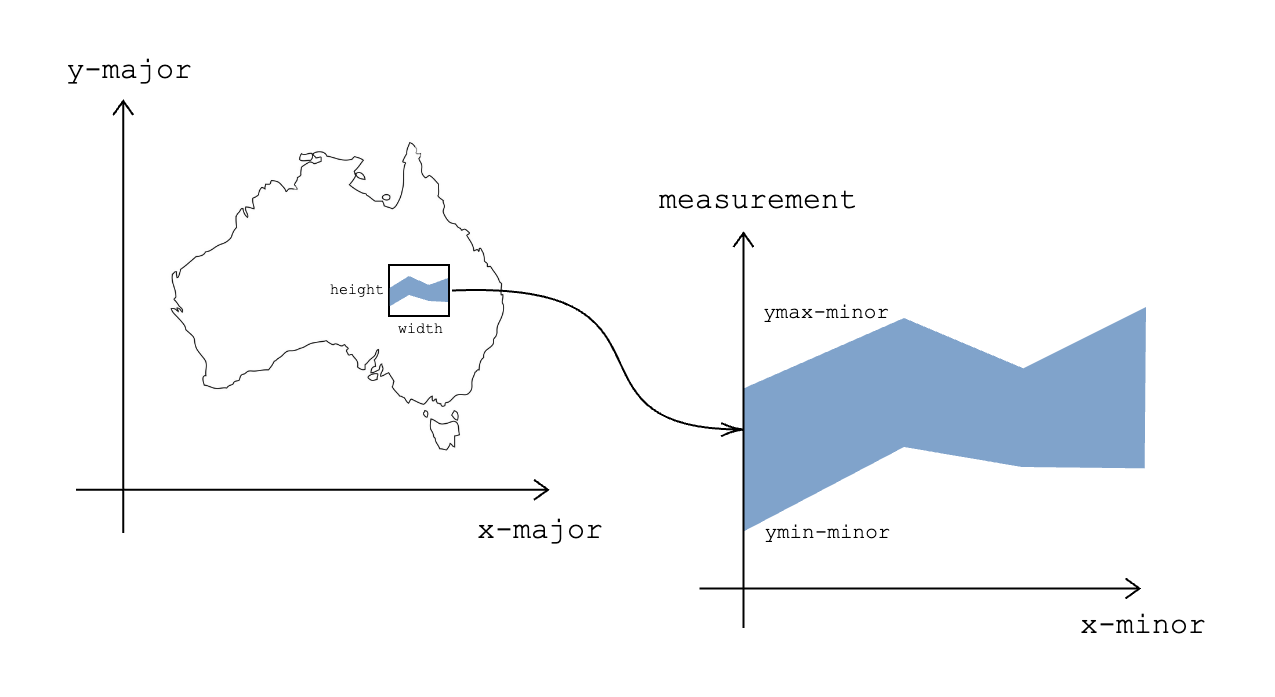
\includegraphics{figures/diagram-transformation.png}
The construction of glyph map (as described in Wickham et al. (2012)) involve a linear mix of two structure component of the data: spatial location and data value. The spatial location is the major axes are latitude (\(y_{major}\)) and longitude (\(x_{minor}\)), and the minor axes are time (\(x_minor\)) and some measurement (\(ymax_{minor}\) and \(ymin_{minor}\)). For \texttt{geom\_segment\_glyph} the aesthetic would be \(y_{minor}\) and \(yend_{minor}\). Once the minor axes are rescaled to {[}-1,1{]}, the final coordinates (\(x\),\(ymin\), \(ymax\)) for ribbon glyph are the linear combination, given by:

\(x = x_{major} + \frac{width}{2}.x_{minor}\)
\(ymin = y_{major} + \frac{height}{2}.ymin_{minor}\)
\(ymax = y_{major} + \frac{height}{2}.ymax_{minor}\)

Similarly, the coordinates for segment glyph are given by:

\(x = x_{major} + \frac{width}{2}.x_{minor}\)
\(y = y_{major} + \frac{height}{2}.y_{minor}\)
\(yend = y_{major} + \frac{height}{2}.yend_{minor}\)

(\ldots)

\hypertarget{aesthetics}{%
\subsubsection{Aesthetics}\label{aesthetics}}

sugarglider provides the same aesthetics for geom\_glyph\_ribbon() and geom\_glyph\_segment() as those available in geom\_ribbon() or geom\_segment(), while also introducing additional unique options.

\hypertarget{parameters}{%
\subsubsection{Parameters}\label{parameters}}

\hypertarget{interactivity}{%
\subsubsection{Interactivity}\label{interactivity}}

\hypertarget{examples}{%
\subsubsection{Examples}\label{examples}}

\hypertarget{application}{%
\section{Application}\label{application}}

Five examples are selected to demonstrate various features of the sugarglider package: (1) Creating a ribbon glyph map to visualize annual fluctuations in minimum and maximum daily patronage for each train station, revealing seasonal trends. (2) Using glyph segments to compare patronage on typical weekdays versus weekends at different stations, enabling insights for optimizing service schedules. (3) Utilizing glyph ribbons to represent variations in patronage during distinct peak periods---AM peak, interpeak, PM peak, and late PM hours---across stations. (4) Displaying differences in patronage across transportation modes (Metro, VLine, or both) using glyph segments, identifying capacity imbalances. Lastly, (5) Employing glyph ribbons to compare public and school holiday patronage against regular days, aiding in scheduling and resource planning.

\hypertarget{yearly-patronage-changes-by-station}{%
\subsubsection{Yearly Patronage Changes by Station}\label{yearly-patronage-changes-by-station}}

\hypertarget{weekday-vs.-weekend-patronage}{%
\subsubsection{Weekday vs.~Weekend Patronage}\label{weekday-vs.-weekend-patronage}}

\hypertarget{patronage-during-different-peak-times}{%
\subsubsection{Patronage During Different Peak Times}\label{patronage-during-different-peak-times}}

\hypertarget{patronage-variations-by-transportation-mode}{%
\subsubsection{Patronage Variations by Transportation Mode}\label{patronage-variations-by-transportation-mode}}

\hypertarget{public-and-school-holiday-patronage-vs.-regular-days}{%
\subsubsection{Public and School Holiday Patronage vs.~Regular Days}\label{public-and-school-holiday-patronage-vs.-regular-days}}

\hypertarget{discussion}{%
\section{Discussion}\label{discussion}}

\hypertarget{acknowledgements}{%
\section{Acknowledgements}\label{acknowledgements}}

\hypertarget{references}{%
\section*{References}\label{references}}
\addcontentsline{toc}{section}{References}

\hypertarget{refs}{}
\begin{CSLReferences}{1}{0}
\leavevmode\vadjust pre{\hypertarget{ref-wickham2012glyph}{}}%
Wickham, Hadley, Heike Hofmann, Charlotte Wickham, and Dianne Cook. 2012. {``Glyph-Maps for Visually Exploring Temporal Patterns in Climate Data and Models.''} \emph{Environmetrics} 23 (5): 382--93.

\leavevmode\vadjust pre{\hypertarget{ref-JSSv110i07}{}}%
Zhang, H. Sherry, Dianne Cook, Ursula Laa, Nicolas Langrené, and Patricia Menéndez. 2024. {``Cubble: An r Package for Organizing and Wrangling Multivariate Spatio-Temporal Data.''} \emph{Journal of Statistical Software} 110 (7): 1--27. \url{https://doi.org/10.18637/jss.v110.i07}.

\end{CSLReferences}


\address{%
Maliny Po\\
Monash University\\%
Department of Econometrics and Business Statistics\\ Melbourne, Australia\\
%
%
\textit{ORCiD: \href{https://orcid.org/0009-0008-4686-6631}{0009-0008-4686-6631}}\\%
\href{mailto:malinypo12@gmail.com}{\nolinkurl{malinypo12@gmail.com}}%
}

\address{%
Dianne Cook\\
Monash University\\%
Department of Econometrics and Business Statistics\\ Melbourne, Australia\\
%
%
\textit{ORCiD: \href{https://orcid.org/0000-0002-3813-7155}{0000-0002-3813-7155}}\\%
\href{mailto:dicook@monash.edu}{\nolinkurl{dicook@monash.edu}}%
}
